\documentclass[10pt,a4paper]{article}

\usepackage{fontspec}
\usepackage{polyglossia}
\setmainlanguage{english}
\setotherlanguage{hindi}
\newfontfamily\devanagarifont[Script=Devanagari]{Noto Sans Devanagari}
\usepackage{geometry}
\geometry{top=0.55in,bottom=0.55in,left=0.65in,right=0.65in}
\usepackage{graphicx}
\newcommand{\attimg}[2]{%
  \begin{minipage}[t]{0.32\textwidth}\centering
    \includegraphics[width=\linewidth,height=0.205\textheight,keepaspectratio]{#1}\par
    \vspace{2pt}{\scriptsize #2}
  \end{minipage}%
}
\usepackage{float}
\usepackage{booktabs}
\usepackage{longtable}
\usepackage{array}
\usepackage{tabularx}
\usepackage{listings}
\usepackage{xcolor}
\usepackage{amsmath}
\usepackage{hyperref}
\usepackage{enumitem}
\usepackage{caption}
\captionsetup{font=small,skip=3pt}
\usepackage{fancyhdr}

\hypersetup{colorlinks=true,linkcolor=blue,urlcolor=blue,citecolor=blue}
\setlength{\parindent}{0pt}
\setlength{\parskip}{0.25em}
\setlist[itemize]{leftmargin=*,itemsep=1pt,topsep=2pt,parsep=0pt}
\setlist[enumerate]{leftmargin=*,itemsep=1pt,topsep=2pt,parsep=0pt}
\lstset{basicstyle=\ttfamily\footnotesize,breaklines=true,frame=single,columns=fullflexible,aboveskip=4pt,belowskip=4pt}

\setlength{\headheight}{14pt}
\usepackage{titlesec}
\titlespacing*{\section}{0pt}{7pt}{3pt}
\titlespacing*{\subsection}{0pt}{5pt}{2pt}
\titlespacing*{\subsubsection}{0pt}{4pt}{1pt}
\setlength{\textfloatsep}{6pt plus 2pt minus 2pt}
\setlength{\floatsep}{5pt plus 2pt minus 2pt}
\setlength{\intextsep}{5pt plus 2pt minus 2pt}
\renewcommand{\arraystretch}{0.88}
\setlength{\tabcolsep}{3pt}
\pagestyle{fancy}
\fancyhf{}
\lhead{LLM Project -- Cumulative Final Report}
\rhead{\thepage}

\title{Language Modelling Individual Project Report}
\author{}
\date{}

\begin{document}
\maketitle
\section{Phase-1 Report}

\subsection{Dataset Accumulation}
\subsubsection{Prebuilt corpus}
\begin{enumerate}
\item Sangraha Nepali Corpus - Extracted 500M words
\item Sangraha Hindi Corpus - Extracted 500M words
\end{enumerate}

\subsubsection{Manual collection}
\paragraph{Consideration}
\begin{enumerate}
\item NewsPaper Scraping
\item Government sites Scraping
\item Literature scraping (if possible and if necessary)
\item Open subtitles (seems to be a good idea)
\end{enumerate}

\paragraph{Actually done}
Data extraction from common crawl which includes all kind
of scraping of the web over various domains.

Performed extraction of the URLs using the duckdb database and
got the warc record offsets and later extracted the relevant
text out of these sites using trafilatura efficiently.

\subsection{Cleaning and Pre-processing}
\begin{enumerate}
\item Remove the extremely short docs. (like less than 100 words may be)
\item Remove Garbage docs (like 404 error or loading etc.,)
\item Remove repetitive docs (may be using hashing)
\item Unicode normalization (something like NFC)
\item Language identification using cld2 or 3 but may not necessary as common crawl already runs cld2
\item Score devanagri script ratio in the docs. (threshold like > 80 or > 90)
\item Remove gibberish as well
\item Character level quality filtering (give quality scoring based on these)
\end{enumerate}
\begin{itemize}
\item alphabetic character ratio
\item digits ratio
\item punctuation ratio
\item weird unicode ratio
\item repeated characters ratio
\end{itemize}
\begin{enumerate}
\item Normalize whitespaces (keep paragraph seperation or not ?)
\item Don't overclean punctuation and also normalize quotes
\item Normalize the english digits and devanagri ones (is there a reason to do or not do this ?)
\item Handle things like the Purna Viram (|) and Full Stop (.).
\item Replace URLs with \textbackslash\{\}<URL\textbackslash\{\}> may be for emails as well
\item Deduplication (remember to include the manual one in case of exact deduplication of records or something)
\end{enumerate}
\begin{itemize}
\item Paragraph dedup
\item Near duplicate removal using MinHash (sentence level as well)
\item Exact dedup
\end{itemize}
\begin{enumerate}
\item Perplexity based filtering (optional)
\item Once the document are clean, splitting them into sentences (may or may not be needed)
\item Safety filtering on the content
\end{enumerate}

\subsubsection{Hindi Pre-processing runs}
With Deduplication
\begin{lstlisting}
python3 ../cleaning/pipeline.py --input combined_hindi_corpus_copy.jsonl --output cleaned.jsonl
\end{lstlisting}

\begin{lstlisting}
======================================================================
FINAL DATASET
======================================================================

TRAIN
  Total words:     357,154,414
  Estimated tokens:500,016,180
  Manual:          71,193,055
  Sangraha:        285,961,359
  Manual ratio:    19.933%

VALIDATION
  Total words:     70,867,645
  Estimated tokens:99,214,703
  Manual:          14,126,837
  Sangraha:        56,740,808
  Manual ratio:    19.934%

TEST
  Total words:     70,852,283
  Estimated tokens:99,193,196
  Manual:          14,118,622
  Sangraha:        56,733,661
  Manual ratio:    19.927%

======================================================================
FILES
======================================================================
splits/train.jsonl
splits/validation.jsonl
splits/test.jsonl
\end{lstlisting}

\subsubsection{Nepali runs}
With Deduplication
\begin{lstlisting}
python3 ../cleaning/pipeline.py --input combined_nepali_corpus_copy.jsonl --output cleaned2.jsonl
\end{lstlisting}
\begin{lstlisting}
======================================================================
FINAL DATASET
======================================================================

TRAIN
  Total words:     357,143,405
  Estimated tokens:500,000,767
  Manual:          66,614,806
  Sangraha:        290,528,599
  Manual ratio:    18.652%

VALIDATION
  Total words:     70,507,150
  Estimated tokens:98,710,010
  Manual:          13,151,850
  Sangraha:        57,355,300
  Manual ratio:    18.653%

TEST
  Total words:     70,503,406
  Estimated tokens:98,704,768
  Manual:          13,149,352
  Sangraha:        57,354,054
  Manual ratio:    18.651%

======================================================================
FILES
======================================================================
splits/train.jsonl
splits/validation.jsonl
splits/test.jsonl
\end{lstlisting}

\subsection{Tokenization report}
Chose unigram tokenizer for both as it seemed better to do a top down approach with all the matras and halants and all.
\subsubsection{Nepali}
\paragraph{Evaluation Summary}
\begin{center}
\small
\begin{longtable}{l l l l l l l l l}
\toprule
Dataset & Vocab & Words & Tokens & UNK & Fertility & Chars/Tok & UNK Rate & UNK Records \\
\midrule
\endhead
test & 4,000 & 70,503,406 & 133,766,591 & 0 & 1.897307 & 2.8894 & 0.000000\% & 0 \\
test & 6,000 & 70,503,406 & 122,105,099 & 0 & 1.731904 & 3.1654 & 0.000000\% & 0 \\
test & 8,000 & 70,503,406 & 115,490,552 & 0 & 1.638085 & 3.3467 & 0.000000\% & 0 \\
test & 10,000 & 70,503,406 & 111,130,811 & 0 & 1.576247 & 3.4780 & 0.000000\% & 0 \\
test & 12,000 & 70,503,406 & 108,119,964 & 0 & 1.533542 & 3.5748 & 0.000000\% & 0 \\
test & 16,000 & 70,503,406 & 103,782,720 & 0 & 1.472024 & 3.7242 & 0.000000\% & 0 \\
validation & 4,000 & 70,507,150 & 133,606,342 & 0 & 1.894933 & 2.8919 & 0.000000\% & 0 \\
validation & 6,000 & 70,507,150 & 121,961,162 & 0 & 1.729770 & 3.1681 & 0.000000\% & 0 \\
validation & 8,000 & 70,507,150 & 115,375,770 & 0 & 1.636370 & 3.3489 & 0.000000\% & 0 \\
validation & 10,000 & 70,507,150 & 111,019,573 & 0 & 1.574586 & 3.4803 & 0.000000\% & 0 \\
validation & 12,000 & 70,507,150 & 108,021,863 & 0 & 1.532070 & 3.5769 & 0.000000\% & 0 \\
validation & 16,000 & 70,507,150 & 103,688,016 & 0 & 1.470603 & 3.7264 & 0.000000\% & 0 \\
\bottomrule
\end{longtable}
\end{center}

\begin{figure}[htbp]
\centering
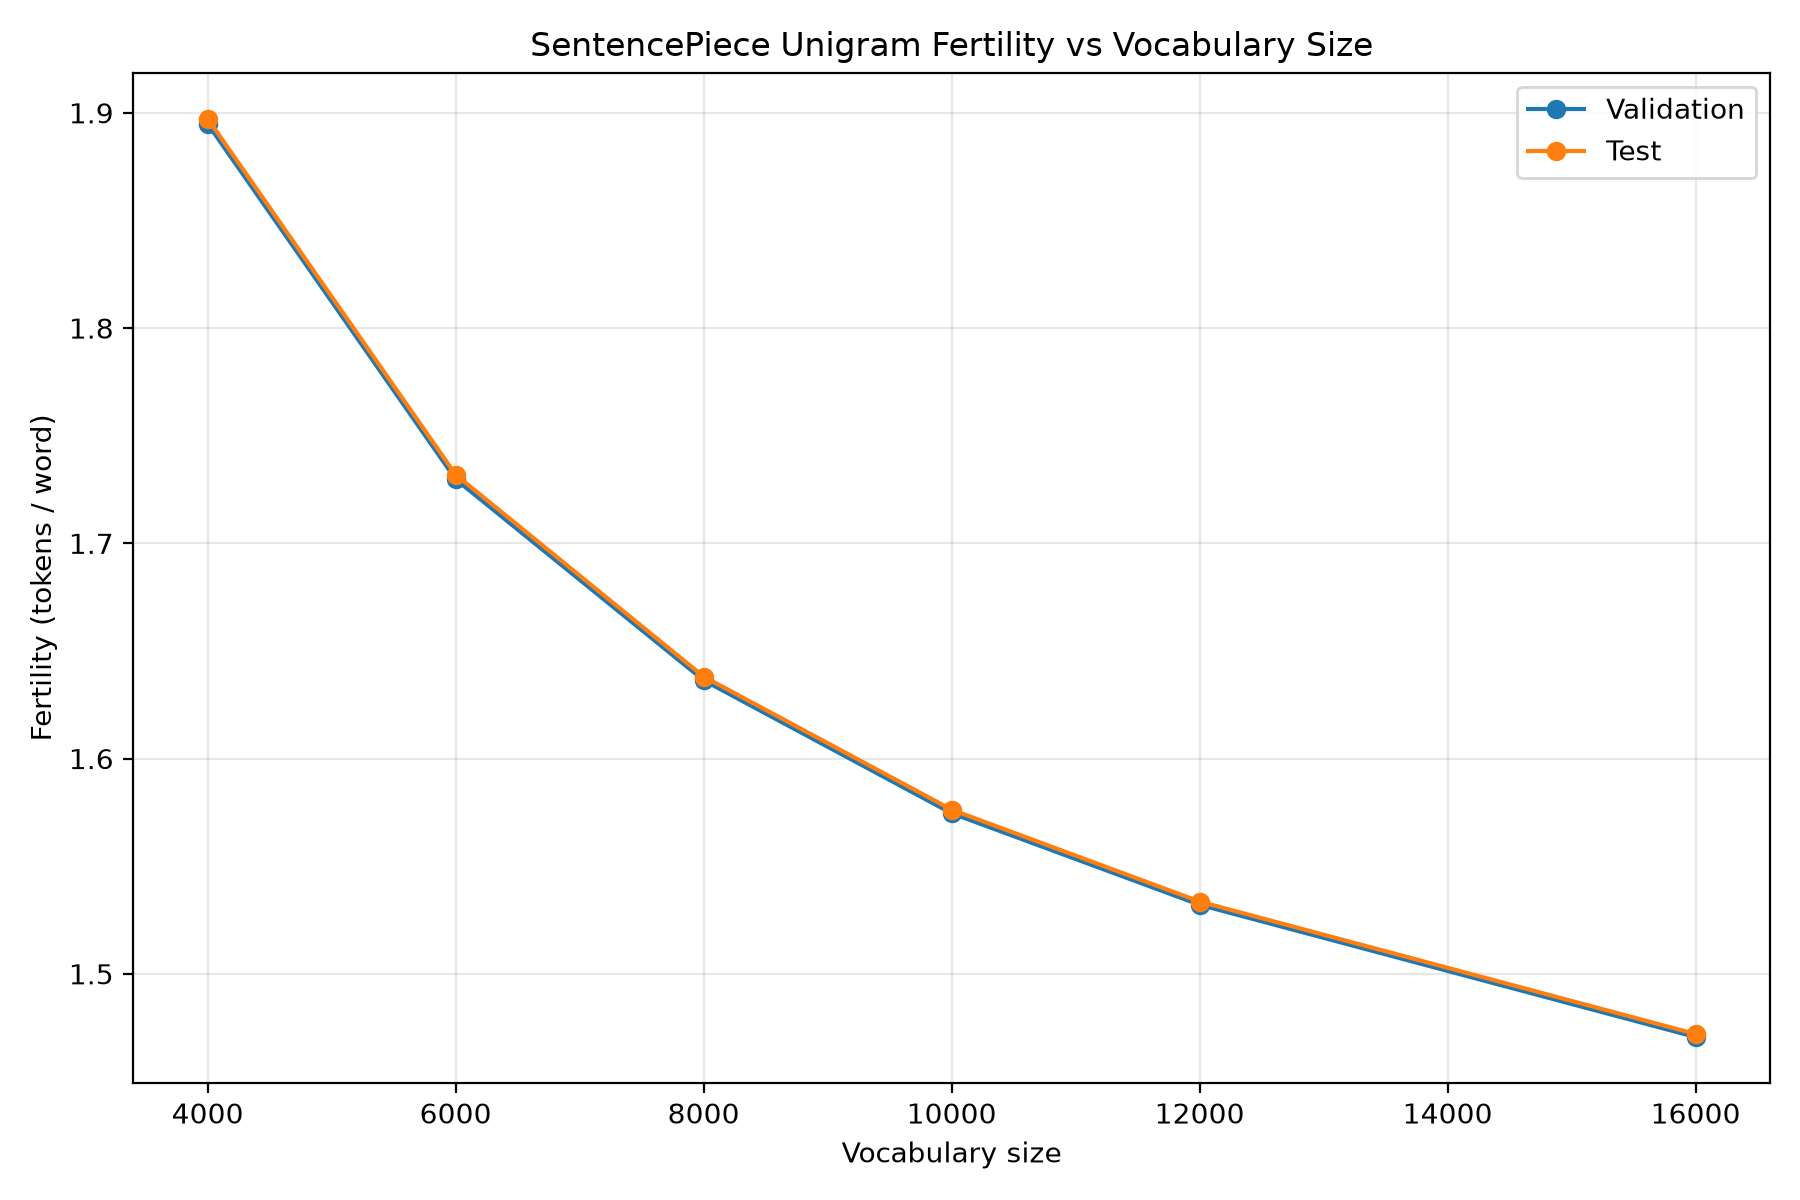
\includegraphics[width=0.68\textwidth]{./nepali/tokenizers/evaluation/fertility_vs_vocab.png}
\caption{Fertility vs Vocab Size}
\end{figure}

\paragraph{For the chosen 10K vocab model (keeping the model parameter constraint in mind)}

\subsubsection{Hindi}
\paragraph{Evaluation Summary}
\begin{center}
\small
\begin{longtable}{l l l l l l l l l}
\toprule
Dataset & Vocab & Words & Tokens & UNK & Fertility & Chars/Tok & UNK Rate & UNK Records \\
\midrule
\endhead
test & 4,000 & 70,852,283 & 118,021,659 & 0 & 1.665742 & 2.4996 & 0.000000\% & 0 \\
test & 6,000 & 70,852,283 & 109,564,214 & 0 & 1.546375 & 2.6926 & 0.000000\% & 0 \\
test & 8,000 & 70,852,283 & 104,917,160 & 0 & 1.480787 & 2.8118 & 0.000000\% & 0 \\
test & 10,000 & 70,852,283 & 101,746,041 & 0 & 1.436031 & 2.8995 & 0.000000\% & 0 \\
test & 12,000 & 70,852,283 & 99,535,951 & 0 & 1.404838 & 2.9638 & 0.000000\% & 0 \\
test & 16,000 & 70,852,283 & 96,576,460 & 0 & 1.363068 & 3.0547 & 0.000000\% & 0 \\
validation & 4,000 & 70,867,645 & 117,738,665 & 0 & 1.661388 & 2.5030 & 0.000000\% & 0 \\
validation & 6,000 & 70,867,645 & 109,314,423 & 0 & 1.542515 & 2.6959 & 0.000000\% & 0 \\
validation & 8,000 & 70,867,645 & 104,682,347 & 0 & 1.477153 & 2.8152 & 0.000000\% & 0 \\
validation & 10,000 & 70,867,645 & 101,519,763 & 0 & 1.432526 & 2.9029 & 0.000000\% & 0 \\
validation & 12,000 & 70,867,645 & 99,334,274 & 0 & 1.401687 & 2.9668 & 0.000000\% & 0 \\
validation & 16,000 & 70,867,645 & 96,401,411 & 0 & 1.360302 & 3.0570 & 0.000000\% & 0 \\
\bottomrule
\end{longtable}
\end{center}

\begin{figure}[htbp]
\centering
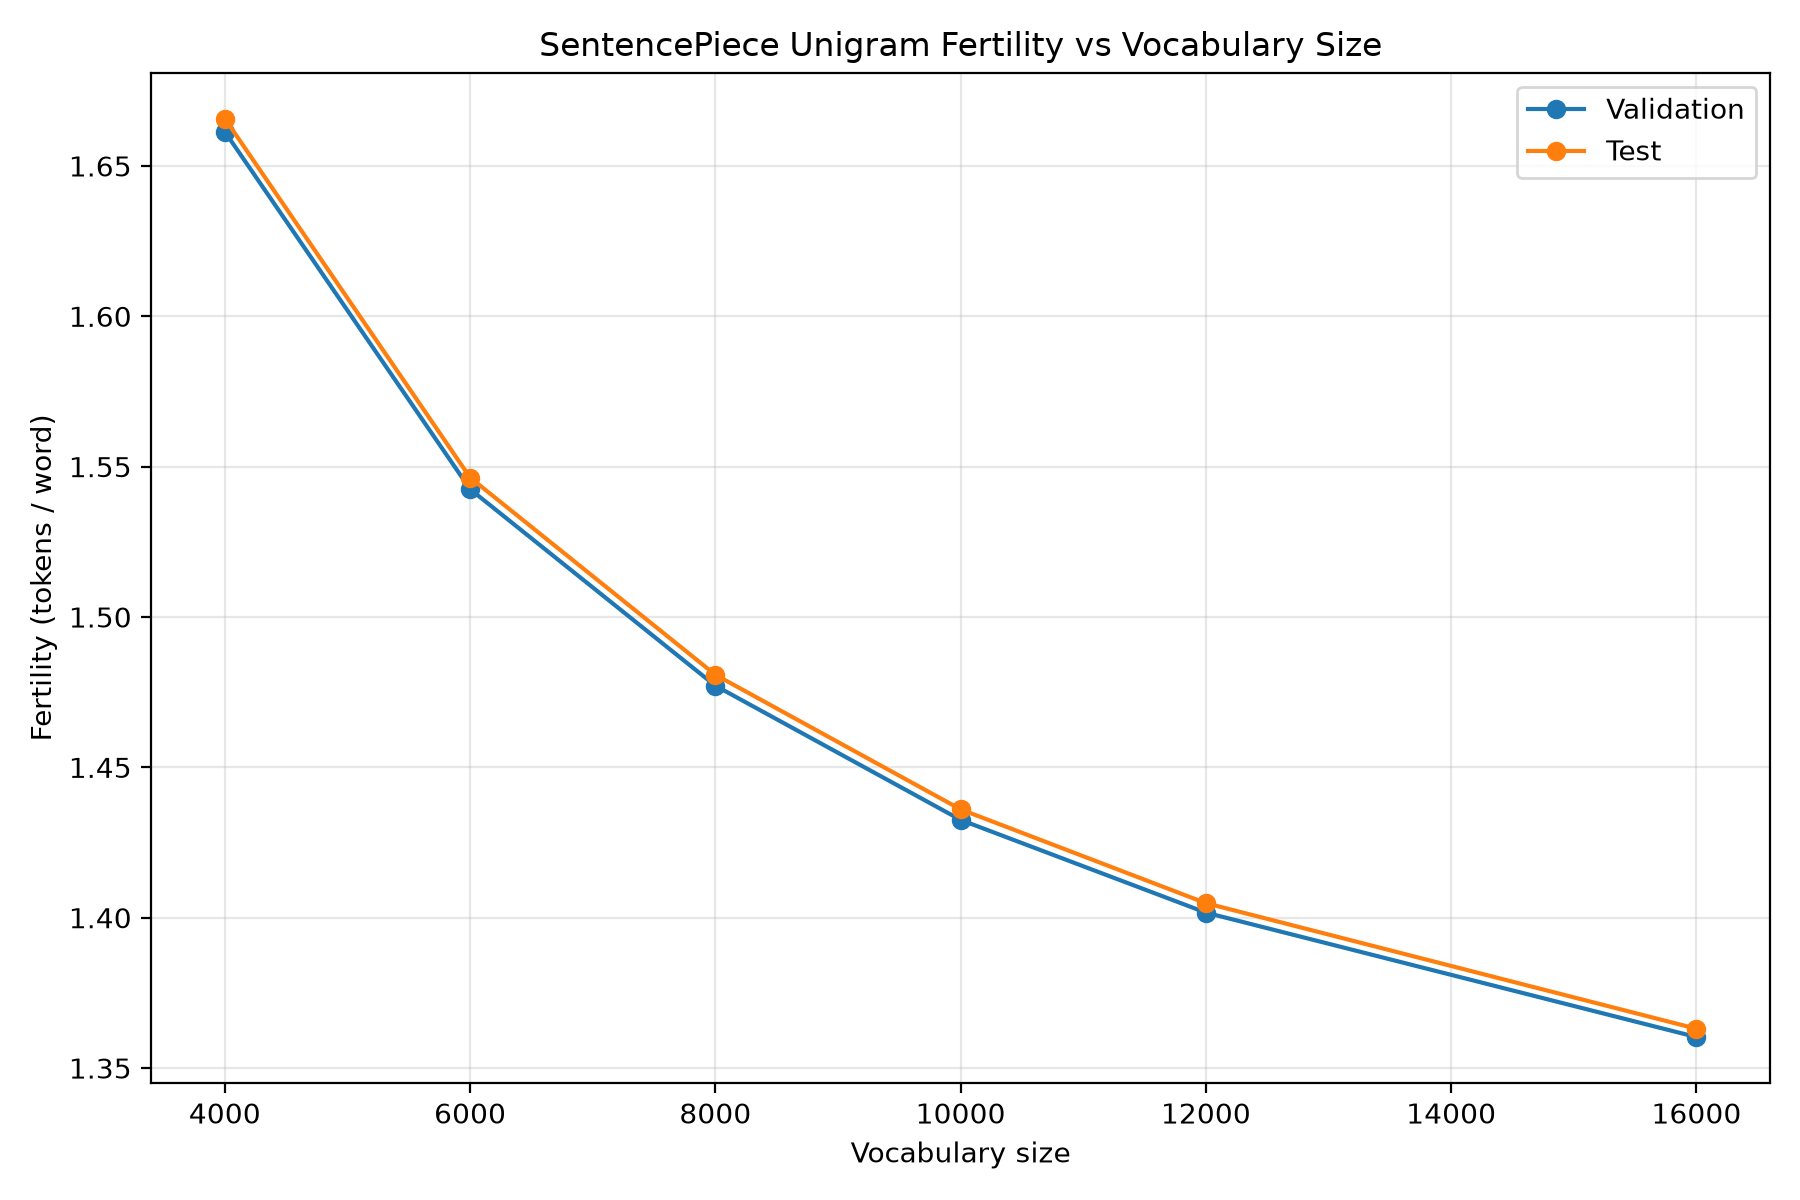
\includegraphics[width=0.68\textwidth]{./hindi/tokenizers/evaluation/fertility_vs_vocab.png}
\caption{Fertility vs Vocab Size}
\end{figure}


\paragraph{For the chosen 8K vocab model (keeping the model parameter constraint in mind)}

\section{Phase-2 Report}

\subsection{WANDB training stuff}

\subsubsection{Hindi}
\begin{figure}[htbp]
\centering
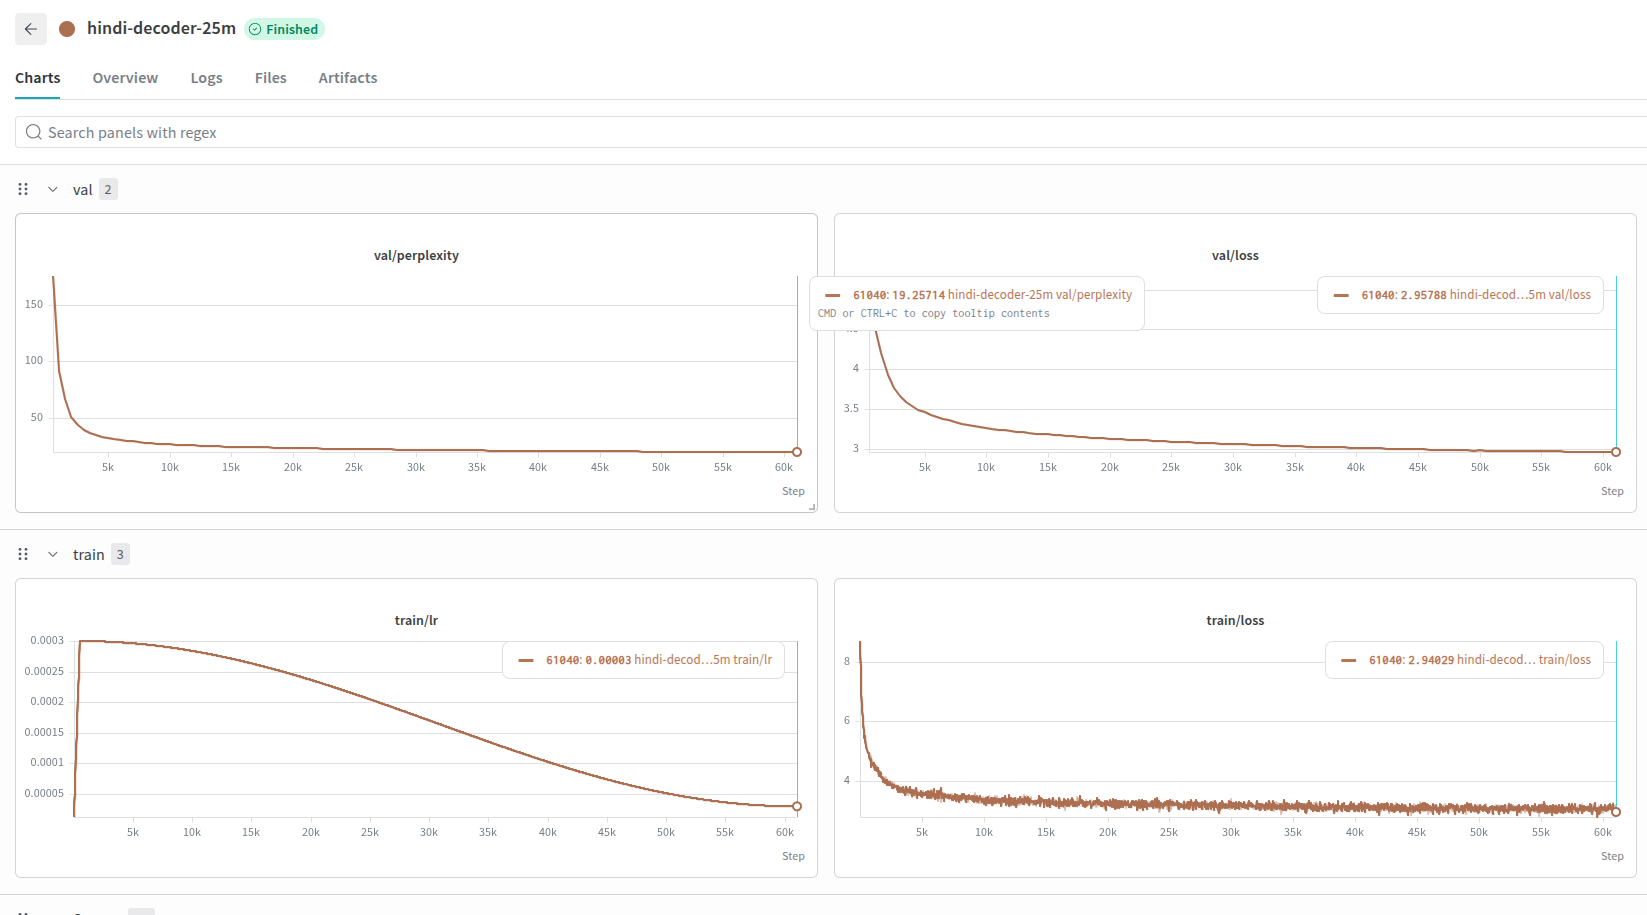
\includegraphics[width=0.68\textwidth]{./wandb_hindi.png}
\caption{}
\end{figure}

\subsubsection{Nepali}
\begin{figure}[htbp]
\centering
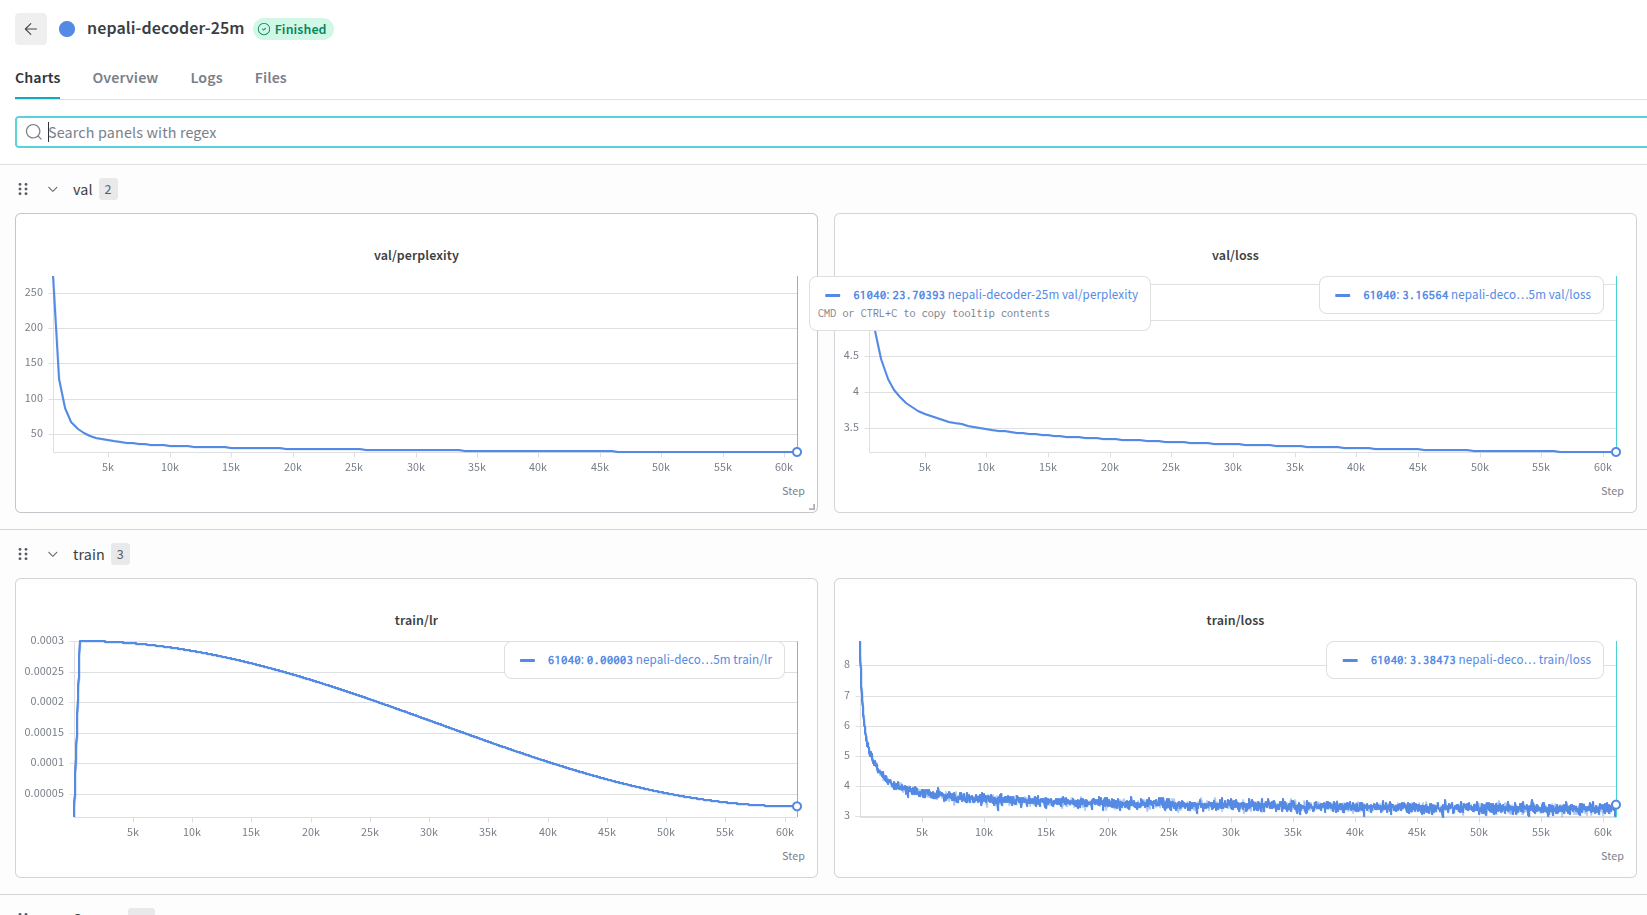
\includegraphics[width=0.68\textwidth]{./wandb_nepali.png}
\caption{}
\end{figure}

\subsection{2.2 Configuration and Reporting}

\textbf{Hyperparameters (Model H \& Model L)}:
\begin{itemize}
\item \textbf{d\_model (dimension)}: 384
\item \textbf{Number of layers}: 12
\item \textbf{Number of heads}: 6
\item \textbf{Feed-forward width (d\_ff)}: 1600
\item \textbf{Context length}: 512
\item \textbf{Dropout}: 0.1
\item \textbf{Vocabulary Size}: 8,000 (Model H - Hindi) / 10,000 (Model L - Nepali)
\end{itemize}

\textbf{Exact Parameter Count}:
\begin{itemize}
\item \textbf{Model H (Hindi)}: 24,956,928 trainable parameters
\item \textbf{Model L (Nepali)}: 25,724,928 trainable parameters
\end{itemize}

\emph{Note: The input embedding layer is tied to the output projection layer.}

\textbf{Depth/Width Trade-off Justification}:
Given the constraint of approximately 25M parameters, I have chosen a deep architecture with 12 layers and a model dimension of 384 to balance that. The idea is that the increased depth would allow the model to learn more abstract relations and hierarchical features, while making sure the moderate width still provides enough representational capacity.

\textbf{Component Explanations}:
\begin{itemize}
\item \textbf{Rotary Position Embedding (RoPE)}: Instead of absolute positional embeddings, the models utilize RoPE, which encodes position information multiplicatively by rotating the query and key representations (Shape of angles: \texttt{[max\_seq\_len, dhead/2]}). Thus, capturing relative positional information effectively with no parameter overhead. Also, there is no maximum sequence length constraint as in absolute positional embeddings.
\item \textbf{Multi-Head Attention (Causal Masking)}: To emperically verify the causal masking, I have given a random token sequence to the model and later changed the \texttt{t+1} token. The logits till position \texttt{t} remained unchanged with an max absolute difference \texttt{0.0}, confirming that the model cannot attend to future tokens. But, the logits at postion \texttt{t+1} changed with max absolute difference \texttt{0.66}. (In this run t = 25)
\item \textbf{Layer Normalization}: Chose to apply pre-norm, as it helps to keep the gradient signal stable for deep networks. (Especially here we are using 12 layers.)
\item \textbf{Output Embedding / Projection}: I have tied the input and output embedding matrices together, to save the number of parameters. To be exact, it saves around \texttt{512 * vocab\_size} parameters. That is approximately \texttt{4.1M} parameters for Model H (Hindi) and \texttt{5.12M} parameters for Model L (Nepali).
\end{itemize}

\subsection{2.3 Language Modeling and Attention Evaluation}

\subsubsection{Intrinsic Language-Modeling Metrics}

\begin{center}
\small
\begin{longtable}{l l l}
\toprule
Metric & Model H (Hindi) & Model L (Nepali) \\
\midrule
\endhead
Validation Cross-Entropy Loss & 2.97 & 3.17 \\
Validation Perplexity & 19.58 & 23.75 \\
Validation BPB & 0.480 & 0.422 \\
Test Cross-Entropy Loss & 3.00 & 3.15 \\
Test Perplexity & 20.13 & 23.34 \\
Test BPB & 0.485 & 0.416 \\
\bottomrule
\end{longtable}
\end{center}

\textbf{Discussion on the Gap}:
Model L (Nepali) has higher perplexity than Model H (Hindi) on the test split (23.34 vs 20.13). But, these can't be compared directly because both the models use tokenizers of different vocabulary sizes. Model L nevertheless obtains lower BPB (0.416 vs 0.485). Model L's (Nepali) tokenizer achieves a fertility of 1.57 and Model H's (Hindi) tokenizer achieves a fertility of 1.47. Thus, Model L is more efficient in terms of byte level compression. This could be due to the quality of the data for Nepali as compared to Hindi. I think for Hindi there is possibility of contamination with many other north Indian languages as well as the dataset also has more variable content, which might explain the higher BPB. Nepali has less data overall and less variability as well.

\subsubsection{Generation Quality}

\begin{center}
\small
\begin{longtable}{l l l l l l l l}
\toprule
Model & Decoding & BLEU-4 & chrF++ & ROUGE-L & Repeat-3 & Distinct-1 & Distinct-2 \\
\midrule
\endhead
\textbf{Model H} & Greedy & 4.66 & 15.54 & 0.0226 & 0.5907 & 0.1369 & 0.2824 \\
 & T=0.5 & 5.04 & 18.07 & 0.0202 & 0.2705 & 0.1945 & 0.4901 \\
 & T=1.0 & 3.30 & 18.03 & 0.0259 & 0.0218 & 0.3248 & 0.8129 \\
 & T=1.5 & 2.11 & 16.39 & 0.0152 & 0.0010 & 0.4728 & 0.9731 \\
\textbf{Model L} & Greedy & 2.02 & 18.36 & 0.0029 & 0.6014 & 0.1475 & 0.2859 \\
 & T=0.5 & 1.88 & 19.71 & 0.0022 & 0.3129 & 0.2167 & 0.4910 \\
 & T=1.0 & 1.05 & 19.15 & 0.0015 & 0.0237 & 0.3893 & 0.8472 \\
 & T=1.5 & 0.22 & 16.65 & 0.0000 & 0.0010 & 0.5366 & 0.9738 \\
\bottomrule
\end{longtable}
\end{center}

\textbf{Metric Informativeness}:
\begin{itemize}
\item \textbf{BLEU \& ROUGE-L}: Poor metrics for open-ended generation. They demand exact n-gram/subsequence overlap. Thus, they are a poor choice for LLM evaluation where multiple valid continuations exist.
\item \textbf{chrF/chrF++}: It is slightly more robust than BLEU and ROUGE-L because it used character n-grams. This could also be better given that Hindi and Nepali are both morphologically rich languages. But it is still a overlap metric hence bad.
\end{itemize}

\textbf{Fluency and Diversity Diagnostics (Qualitative Notes)}:

The following continuations are sampled from the held-out examples saved by the evaluation script. Each uses a 32-token prefix and generates up to 64 tokens.

\begin{itemize}
\item \textbf{Greedy decoding}: Frequently enters short repetition loops, consistent with the high Repeat-3 values (Hindi: 0.5907; Nepali: 0.6014).
\end{itemize}

\begin{itemize}
\item \textbf{Temperature \$T=0.5\$}: It reduces three-gram repetition substantially relative to greedy decoding (Hindi: 0.2705; Nepali: 0.3129).
\end{itemize}

\begin{itemize}
\item \textbf{Temperature \$T=1.0\$}: This setting largely removes the severe repetition loops (Repeat-3: 0.0218 for Hindi and 0.0237 for Nepali) and has high lexical diversity (Distinct-2: 0.8129 and 0.8472).
\end{itemize}

\begin{itemize}
\item \textbf{Temperature \$T=1.5\$}: This produces the highest diversity (Distinct-2: 0.9731 for Hindi and 0.9738 for Nepali) and near-zero three-gram repetition, but the low BLEU/ROUGE scores and qualitative inspection indicate substantially reduced local coherence.
\end{itemize}

\subsubsection{Attention Analysis}

\textbf{Attention Heatmaps \& Statistics}
\emph{(The generated heatmaps are available in the respective \texttt{attention\_analysis} directories)}

\begin{center}
\attimg{hindi/training/attention_analysis/attention_layer_1.png}{Hindi, layer 1}\hfill
\attimg{hindi/training/attention_analysis/attention_layer_12.png}{Hindi, layer 12}\hfill
\attimg{hindi/training/attention_analysis/attention_entropy.png}{Hindi attention entropy}\\[0.7em]
\attimg{hindi/training/attention_analysis/attention_distance.png}{Hindi attention distance}\hfill
\attimg{nepali/training/attention_analysis/attention_layer_1.png}{Nepali, layer 1}\hfill
\attimg{nepali/training/attention_analysis/attention_layer_12.png}{Nepali, layer 12}\\[0.7em]
\end{center}
\clearpage
\begin{center}
\attimg{nepali/training/attention_analysis/attention_entropy.png}{Nepali attention entropy}\hfill
\attimg{nepali/training/attention_analysis/attention_distance.png}{Nepali attention distance}\hfill
\end{center}


\textbf{Discussion}:
\begin{itemize}
\item \textbf{Local vs. Long-range Heads}: By analyzing attention entropy and mean distance, we observe that early layers (e.g., Layer 1) generally have high entropy (\textasciitilde{}1.6 - 1.9) and moderate attention distances, indicating diffuse, broad attention as the model builds initial token representations.
\item \textbf{Content-based Heads}: In middle-to-late layers (e.g., Layer 9), highly specialized heads emerge. For example, in Model H's Layer 9, Heads 5 and 6 have very low entropy (0.40 and 0.38) but very high mean attention distances (7.3 - 7.5 tokens). These are content-based heads that confidently attend to specific distant tokens (like tracking entities or structural dependencies).
\item \textbf{Positional Heads}: Some heads remain strictly local. In Model L's Layer 3, Head 5 has a mean distance of just 1.65, functioning primarily to look at the immediate preceding token.
\item \textbf{Model H vs. Model L Differences}: Both models exhibit similar layer-wise progression (diffuse -> specialized -> mixed output formulation). Model H tends to develop slightly more distinct low-entropy, long-range heads in Layer 9, while Model L develops them slightly deeper (Layer 11).
\end{itemize}

\section{Phase-3 Report}

\paragraph{1. How did data scale and quality differ between Model H and Model L?}
Model H (Hindi) and Model L (Nepali) had scale and quality wise almost similar datasets, they share the same script so even pre-processing was similar. Although hindi had more data overall by large margin for the scale of our project even Nepali had sufficient data.

\paragraph{2. How do language-modeling and reasoning results compare across the two resource tiers?}
Model H (Hindi) and Model L (Nepali) perform similarly in language modeling, but Model H performs better in reasoning finetuning. This is likely due to more diversity in Hindi dataset compared to Nepali dataset which was predominantly only newspaper articles.

\paragraph{3. What tokenizer / corpus factors most affected the lower-resource model?}
For Nepali I had to go with a larger vocabulary size tokenizer to achieve a smaller fertility comparable to Hindi, also the corpus being small meant I could not be very generous with the pre-processing and cleaning steps.

\paragraph{4. What evidence explains the observed differences?}
The evidence of low diversity for Nepali dataset may be seen in the lower BPB (0.422) compared to Hindi (0.480) and even the Repeat-3 values of Nepali are higher than Hindi.

\subsection{After Fine-tuning metrics}

\paragraph{1. Intrinsic Language-Modeling Metrics (Pre-trained vs. Fine-tuned)}

\begin{center}
\small
\begin{longtable}{l l l l l}
\toprule
Metric & H PT &  H FT &  L PT &  L FT \\
\midrule
\endhead
\textbf{Validation Cross-Entropy Loss} & 2.97 & 3.32 & 3.17 & 3.46 \\
\textbf{Validation Perplexity} & 19.58 & 27.78 & 23.75 & 31.87 \\
\textbf{Validation BPB} & 0.480 & 0.537 & 0.422 & 0.461 \\
\textbf{Test Cross-Entropy Loss} & 3.00 & 3.35 & 3.15 & 3.45 \\
\textbf{Test Perplexity} & 20.14 & 28.43 & 23.34 & 31.44 \\
\textbf{Test BPB} & 0.485 & 0.541 & 0.416 & 0.456 \\
\bottomrule
\end{longtable}
\end{center}

\paragraph{2. Downstream Reasoning and Generation Evaluation (Test Set, N = 600)}

Using generation-based evaluation on the 600 held-out reasoning test instances across relational and comparative reasoning tasks:

\begin{center}
\small
\begin{longtable}{l l l l l}
\toprule
Metric & H PT & H FT & L PT & L FT \\
\midrule
\endhead
\textbf{Logical Accuracy} & 22.17\% & \textbf{85.83\%} & 6.00\% & \textbf{77.17\%} \\
\textbf{Entity Accuracy} & 43.17\% & \textbf{86.50\%} & 22.17\% & \textbf{79.00\%} \\
\textbf{Relation Accuracy} & 59.17\% & \textbf{100.00\%} & 35.33\% & \textbf{99.83\%} \\
\textbf{Ordering Accuracy} & 0.00\% & \textbf{48.78\%} & 0.00\% & \textbf{50.00\%} \\
\textbf{Prompt Echo Rate} & 3.33\% & 10.33\% & 0.33\% & 10.17\% \\
\textbf{Empty Output Rate} & 0.17\% & 0.00\% & 0.00\% & 0.00\% \\
\bottomrule
\end{longtable}
\end{center}

\paragraph{3. Task Breakdown by Question Type}

\subparagraph{Model H (Hindi) Breakdown}
\begin{center}
\small
\begin{longtable}{l l l l l l l l}
\toprule
Question Type & Count & PT Logical Acc & FT Logical Acc & PT Entity Acc & FT Entity Acc & PT Relation Acc & FT Relation Acc \\
\midrule
\endhead
\texttt{compare\_two} & 192 & 33.85\% & \textbf{100.00\%} & 68.75\% & \textbf{100.00\%} & 48.44\% & \textbf{100.00\%} \\
\texttt{largest} & 147 & 38.10\% & \textbf{95.92\%} & 42.86\% & \textbf{95.92\%} & 82.31\% & \textbf{100.00\%} \\
\texttt{smallest} & 110 & 4.55\% & \textbf{85.45\%} & 37.27\% & \textbf{85.45\%} & 6.36\% & \textbf{100.00\%} \\
\texttt{ordering} & 123 & 0.00\% & \textbf{48.78\%} & 1.63\% & \textbf{52.03\%} & 100.00\% & \textbf{100.00\%} \\
\texttt{relation} & 28 & 25.00\% & \textbf{100.00\%} & 75.00\% & \textbf{100.00\%} & 39.29\% & \textbf{100.00\%} \\
\bottomrule
\end{longtable}
\end{center}

\subparagraph{Model L (Nepali) Breakdown}
\begin{center}
\small
\begin{longtable}{l l l l l l l l}
\toprule
Question Type & Count & PT Logical Acc & FT Logical Acc & PT Entity Acc & FT Entity Acc & PT Relation Acc & FT Relation Acc \\
\midrule
\endhead
\texttt{compare\_two} & 303 & 3.96\% & \textbf{98.02\%} & 21.45\% & \textbf{98.35\%} & 17.49\% & \textbf{99.67\%} \\
\texttt{largest} & 96 & 19.79\% & \textbf{64.58\%} & 28.12\% & \textbf{64.58\%} & 63.54\% & \textbf{100.00\%} \\
\texttt{smallest} & 87 & 1.15\% & \textbf{35.63\%} & 32.18\% & \textbf{35.63\%} & 10.34\% & \textbf{100.00\%} \\
\texttt{ordering} & 82 & 0.00\% & \textbf{50.00\%} & 1.22\% & \textbf{62.20\%} & 100.00\% & \textbf{100.00\%} \\
\texttt{relation} & 32 & 12.50\% & \textbf{100.00\%} & 37.50\% & \textbf{100.00\%} & 21.88\% & \textbf{100.00\%} \\
\bottomrule
\end{longtable}
\end{center}

\paragraph{4. Observations \& Findings}
We can see that fine-tuning definitely improved the reasoning performance of the models. Also in a different way it has effected the models to now generate smaller outputs compared to before where they were yapping lengthy responses.

\subsection{Attention Analysis (post-finetune)}

\textbf{Attention Heatmaps \& Statistics}
\emph{(The generated heatmaps are available in the respective \texttt{attention\_analysis\_reasoning} directories)}

\begin{center}
\attimg{hindi/finetuning/attention_analysis_reasoning/attention_layer_1.png}{Hindi, layer 1}\hfill
\attimg{hindi/finetuning/attention_analysis_reasoning/attention_layer_12.png}{Hindi, layer 12}\hfill
\attimg{hindi/finetuning/attention_analysis_reasoning/attention_entropy.png}{Hindi attention entropy}\\[0.7em]
\attimg{hindi/finetuning/attention_analysis_reasoning/attention_distance.png}{Hindi attention distance}\hfill
\attimg{nepali/finetuning/attention_analysis_reasoning/attention_layer_1.png}{Nepali, layer 1}\hfill
\attimg{nepali/finetuning/attention_analysis_reasoning/attention_layer_12.png}{Nepali, layer 12}\\[0.7em]
\end{center}
\clearpage
\begin{center}
\attimg{nepali/finetuning/attention_analysis_reasoning/attention_entropy.png}{Nepali attention entropy}\hfill
\attimg{nepali/finetuning/attention_analysis_reasoning/attention_distance.png}{Nepali attention distance}\hfill
\end{center}


\textbf{Comments}
\begin{itemize}
\item We can see that the attention heatmaps have become more activated now on the comparison tasks, as opposed to before when some heads seemed to be idle.
\item We can see that some heads are particulary focusing on some tokens (likely the entity tokens in comparison). See head 3 layer 12 of Hindi or layer 12 heads of Nepali.
\item Some heads also seem to have become more long range now like head 3 in layer 12 of Hindi.
\item Overall, the attention patterns indicate that the model has learned to better focus on relevant tokens for reasoning tasks post-finetuning.
\end{itemize}

\section{Bonus Report}

\subsection{Ablation: No Positional Embedding vs. RoPE (Hindi)}

This section compares the standard Hindi model (\textbf{Model H}, using Rotary Position Embedding / RoPE) against the bonus Hindi model trained \textbf{without any positional embedding} (NoPE). Both models share the same architecture (12 layers, d\_model=384, 6 heads, 25M parameters) and were trained on the same Hindi corpus. The only difference is the positional encoding scheme.

\subsubsection{Intrinsic Language-Modeling Metrics}

\begin{center}
\small
\begin{longtable}{l l l}
\toprule
Metric & Model H (Hindi, RoPE) & Bonus (Hindi, No Positional Embedding) \\
\midrule
\endhead
\textbf{Validation Cross-Entropy Loss} & 2.97 & 5.09 \\
\textbf{Validation Perplexity} & 19.58 & 162.06 \\
\textbf{Validation BPB} & 0.480 & 0.822 \\
\textbf{Test Cross-Entropy Loss} & 3.00 & 5.11 \\
\textbf{Test Perplexity} & 20.14 & 165.04 \\
\textbf{Test BPB} & 0.485 & 0.825 \\
\bottomrule
\end{longtable}
\end{center}

\begin{quote}
The model without positional embedding achieves dramatically higher perplexity (\textasciitilde{}165 vs \textasciitilde{}20), confirming that positional information is critical for the causal language modeling task at this model scale. Without knowing token order, the model cannot learn coherent sequential structure.
\end{quote}

\subsubsection{Generation Quality Metrics}

Using 100 held-out examples with 32-token prefix, generating up to 64 tokens:

\begin{center}
\small
\begin{longtable}{l l l l l l l l}
\toprule
Decoding & Model & BLEU-4 & chrF++ & ROUGE-L & Repeat-3 & Distinct-1 & Distinct-2 \\
\midrule
\endhead
\textbf{Greedy} & Model H (RoPE) & 2.58 & 21.70 & 0.1454 & 0.4818 & 0.2058 & 0.4088 \\
 & Bonus (No Pos. Emb.) & 0.30 & 5.71 & 0.0338 & 0.2442 & 0.1977 & 0.3907 \\
\textbf{T=0.5} & Model H (RoPE) & 2.77 & 25.01 & 0.1481 & 0.1569 & 0.2974 & 0.6774 \\
 & Bonus (No Pos. Emb.) & 0.19 & 8.90 & 0.0547 & 0.1674 & 0.2982 & 0.6134 \\
\textbf{T=1.0} & Model H (RoPE) & 1.24 & 25.33 & 0.1207 & 0.0044 & 0.4495 & 0.9072 \\
 & Bonus (No Pos. Emb.) & 0.15 & 19.34 & 0.0726 & 0.0010 & 0.5832 & 0.9716 \\
\textbf{T=1.5} & Model H (RoPE) & 0.85 & 22.72 & 0.0780 & 0.0002 & 0.6383 & 0.9864 \\
 & Bonus (No Pos. Emb.) & 0.07 & 20.38 & 0.0471 & 0.0000 & 0.6936 & 0.9980 \\
\bottomrule
\end{longtable}
\end{center}

\subsubsection{Attention heatmaps}
\begin{center}
\attimg{hindi/training/attention_analysis/attention_layer_12.png}{Hindi, layer 12 (RoPE)}\hfill
\attimg{attention_layer_12.png}{Hindi, layer 12 (without positional embeddings)}\hfill
\end{center}

\textbf{Observations}
\begin{itemize}
\item BLEU, ROUGE, chrF++ all are worse significantly for the no-positional-embedding model, indicating lower generation quality.
\item But you can see that in Repeat and Distinct it does better. Showing model struggles in generating a meaningful sequence.
\item Even perplexity wise no-positional embedding model does very badly.
\item You can see that even the attention heatmaps for the heads have changed and are more diffused now for the no-positional-embedding model in comparison.
\item Thus, the positional embeddings are absolutely essential for Transformer based models.
\end{itemize}


\end{document}
